\chapter{Introducción}
\label{cap:introduccion}

% \chapterquote{La revolución industrial y sus consecuencias han sido un desastre para la raza humana}{Theodore Kaczynski}

En los últimos años el avance de tecnologías inmersivas como la \gls{vr} ha proporcionado un gran cambio en la forma en la que los usuarios interactúan en los entornos digitales.
Grandes empresas como Meta o Apple han apostado por el desarrollo de hardware para estas tecnologías con el lanzamiento de Meta Quest 3 y Apple Vision Pro, así como con la creación de plataformas de interacción social en el \gls{metaverso} con el desarrollo de Meta Horizon Worlds.
Esta tecnología ha abierto nuevas oportunidades para explorar modos de comunicación más naturales en espacios virtuales mediante la comunicación no verbal.

La comunicación no verbal es aquella que no se basa en el uso de palabras, sino que utiliza las imágenes y los gestos para transmitir un mensaje.
En nuestro día a día representa una parte esencial de las comunicaciones humanas, sin embargo su representación en entornos virtuales es más limitada y dependiente de acciones predefinidas como animaciones o ``emotes'' ya introducidos en el juego.
Es por esto que el desarrollo de herramientas que permitan capturar e interpretar en tiempo real estos gestos constituye un gran paso hacia entornos virtuales más expresivos y realistas.


\section{Motivación}
Como se ha mencionado en la introducción, el uso de la comunicación no verbal en entornos virtuales está limitado y prefijado por el diseño de éstos, limitando una parte fundamental de la forma de expresarse cotidiana de los humanos.
Debido a esto y como podemos ver en artículos como \cite{Neverova} o \cite{VRHANDS} la detección de gestos es un campo de estudio que actualmente se está explorando para intentar resolver este problema.
Por estas razones es interesante investigar formas de ampliar esta representación de la comunicación no verbal para que la comunicación entre usuarios y \glspl{npc} sea más natural.

Es por este motivo que este trabajo se inscribe dentro de la línea de investigación de herramientas que puedan reconocer gestos realizados por un usuario mediante un traje de captura de movimiento con el fin de crear entornos virtuales más inmersivos y naturales para los usuarios.

Por otra parte, es necesaria una gran cantidad de datos para crear modelos de \gls{ia} que permitan crear las herramientas mencionadas.
En el caso de este proyecto, los datos necesarios son una secuencia de coordenadas 3D de posiciones y rotaciones de los huesos del esqueleto a lo largo de las animaciones, por lo que los datos que se necesitan procesar tienen un tamaño relativamente grande.
Es por esto que es necesario crear modelos complejos que procesen un número significativo de datos de entrada, pero como desarrollaremos a lo largo del trabajo, no ha sido posible encontrar datasets de este tipo de datos.
Como consecuencia de este motivo, una gran aportación de este trabajo en el campo ha sido la creación de un dataset gracias a la extracción de animaciones de un banco especializado en estas y a la captura de movimientos de usuarios.

Vistos estos motivos, se puede concretar que, la carencia de métodos naturales de explotar la comunicación no verbal en entornos virtuales y la falta de datasets de animaciones han motivado los objetivos mencionados y que expandiremos a continuación.
\section{Objetivos}

El objetivo general de este proyecto es la implementación de un modelo de \gls{ia} que, con baja latencia, permita identificar el gesto que se esté realizando con un traje de captura de movimiento en tiempo real, con la intención de mejorar la comunicación no verbal en entornos virtuales.
Para cumplir el objetivo, se han propuesto las siguientes metas durante el desarrollo del trabajo:
\begin{enumerate}
	%\renewcommand{\theenumi}{\alph{enumi}}
	\item Búsqueda de datasets de animaciones que se han considerado relevantes a la hora de comunicarse con un \gls{npc} en un videojuego. Estas animaciones han sido bailar, saludar, señalar, sentarse, pelear y correr.
	\item Extracción automática de las animaciones mencionadas anteriormente de bancos de animaciones y posterior procesamiento.
	\item Extracción de las animaciones mediante la captura de movimiento de un grupo heterogéneo de usuarios.
	\item Implementación, entrenamiento y comparación de distintos modelos de \gls{ia}, tanto redes neuronales (LSTM, CNN y RNN) como modelos de clasificación clásicos (Random Forest)
	\item Implementación de una aplicación final a modo de demostración para enseñar los resultados en \gls{vr} para aumentar el grado de inmersión.
\end{enumerate}

Como gran objetivo secundario y debido a la falta de datasets de animaciones se ha propuesto publicar los datasets resultantes, tanto de las animaciones artificiales como de las capturas de usuarios.

\section{Plan de trabajo}
El plan de trabajo consiste en varios pasos:
\begin{enumerate}
	%\renewcommand{\theenumi}{\alph{enumi}}
	\item Búsqueda de un dataset: generar un dataset lo suficientemente grande con varios ejemplos de gestos como para poder entrenar de forma adecuada diferentes modelos. Este dataset debe estar compuesto en su mayoría por datos de usuarios reales para poder identificar gestos lo más naturales posibles.
	\item Implementación de modelos de \gls{ia}: implementación de varios modelos de \gls{ia} para poder hacer una comparativa entre ellos y decidir cuál es el más adecuado teniendo en cuenta su velocidad de predicción y su precisión. La implementación de dichos modelos debe contener: entrenador, forma de sacar las estadísticas del modelo final, búsqueda de hiperparámetros, generador de matriz de confusión y debe ser acoplable a una interfaz de usuario común a todos los entrenamientos.
	\item Desarrollo de una interfaz de usuario para el entrenamiento y monitorización de los distintos modelos: desarrollo de una interfaz web para que los usuarios con menos experiencia en programación e \gls{ia} puedan entrenar modelos capaces de predecir los gestos que necesiten sin necesidad de modificar el código ni tener que saber como funciona internamente la base de código.
	\item Desarrollo de una aplicación final: desarrollo de una aplicación para las Oculus Quest a forma de demo en la que se conecte al modelo elegido y se pueda ver en tiempo real su uso.
\end{enumerate}

El desarrollo de las tareas y su planificación se puede ver en la figura \ref{fig:diagrama-gantt}.

\begin{figure}[H]
	\centering
	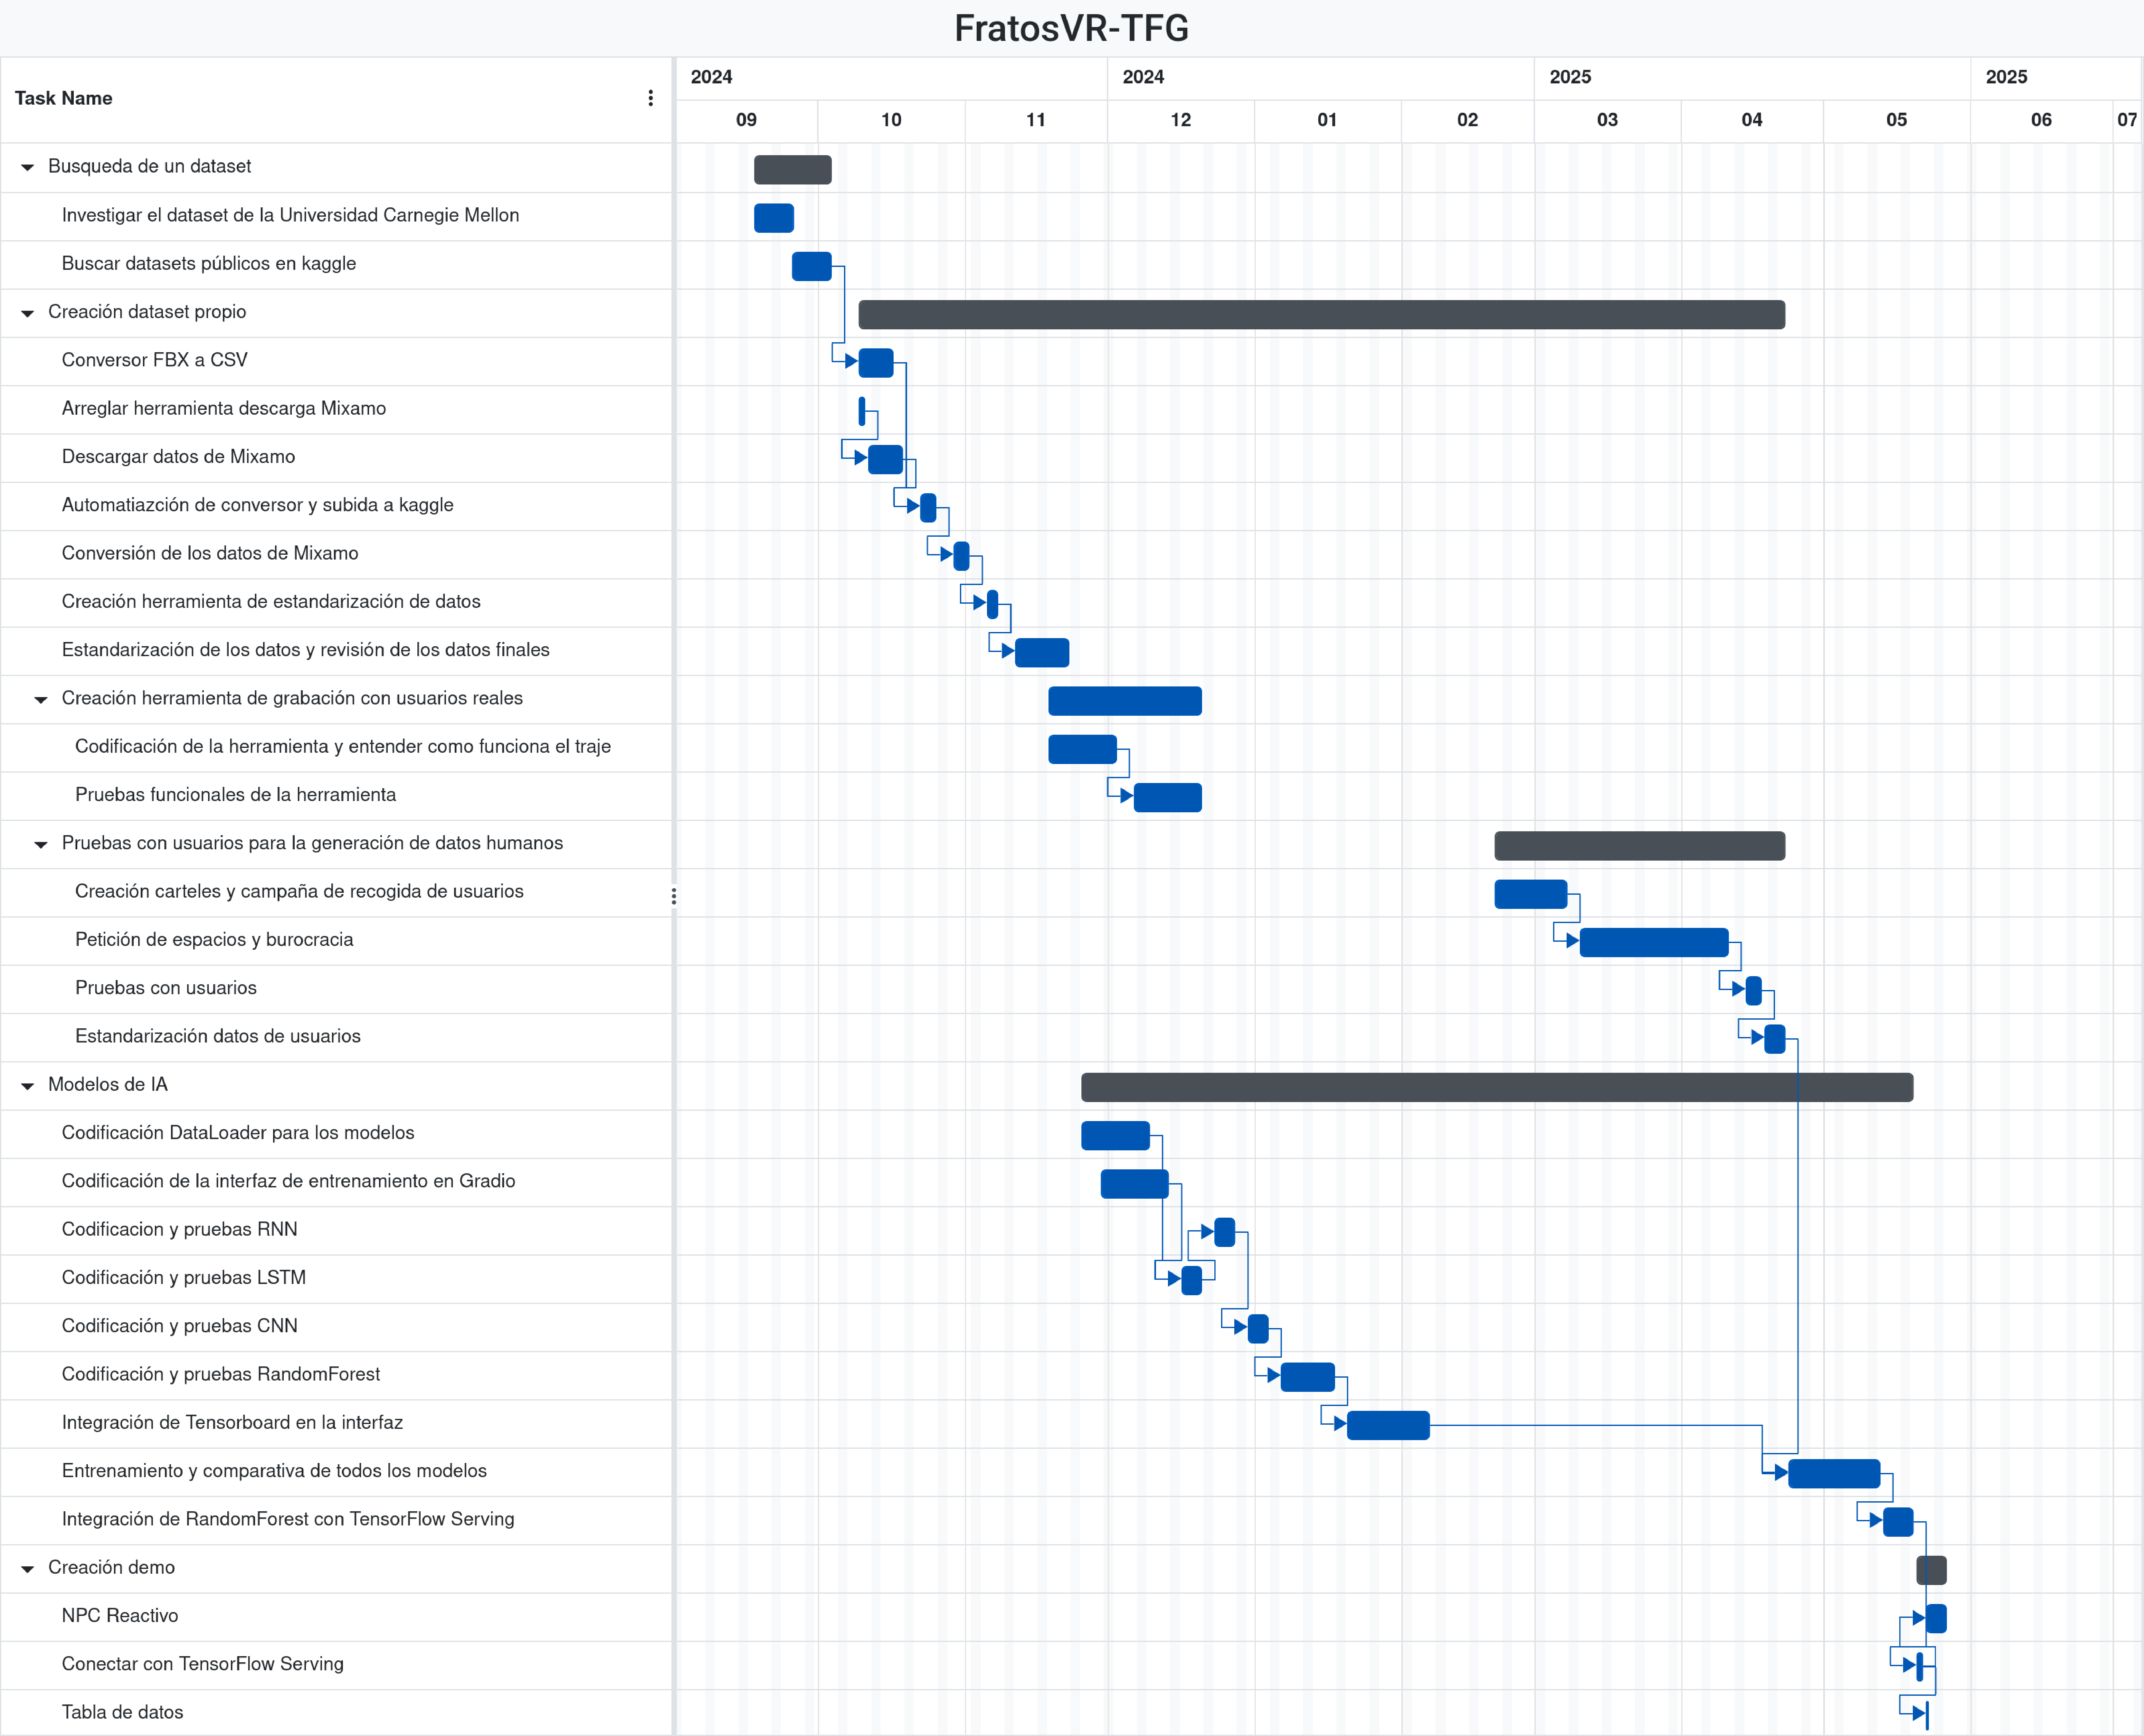
\includegraphics[width=0.91\textwidth]{Imagenes/Vectorial/Diagrama-gannt.pdf}
	\caption{Diagrama de Gantt del proyecto}
	\label{fig:diagrama-gantt}
\end{figure}

